%\documentstyle[epsf,twocolumn]{jarticle}       %LaTeX2.09仕様
\documentclass[twocolumn]{jarticle}     %pLaTeX2e仕様
%%%%%%%%%%%%%%%%%%%%%%%%%%%%%%%%%%%%%%%%%%%%%%%%%%%%%%%%%%%%%%
%%
%%  基本 バージョン
%%
%%%%%%%%%%%%%%%%%%%%%%%%%%%%%%%%%%%%%%%%%%%%%%%%%%%%%%%%%%%%%%%%
\setlength{\topmargin}{-45pt}
%\setlength{\oddsidemargin}{0cm} 
\setlength{\oddsidemargin}{-7.5mm}
%\setlength{\evensidemargin}{0cm} 
\setlength{\textheight}{24.1cm}
%setlength{\textheight}{25cm} 
\setlength{\textwidth}{17.4cm}
%\setlength{\textwidth}{172mm} 
\setlength{\columnsep}{11mm}

\kanjiskip=.07zw plus.5pt minus.5pt


%【節がかわるごとに(1.1)(1.2) …(2.1)(2.2)と数式番号をつけるとき】
%\makeatletter
%\renewcommand{\theequation}{%
%\thesection.\arabic{equation}} %\@addtoreset{equation}{section}
%\makeatother

%\renewcommand{\arraystretch}{0.95} 行間の設定

%%%%%%%%%%%%%%%%%%%%%%%%%%%%%%%%%%%%%%%%%%%%%%%%%%%%%%%%
\usepackage[dvipdfm]{graphicx}   %pLaTeX2e仕様(要\documentstyle ->\documentclass)
%%%%%%%%%%%%%%%%%%%%%%%%%%%%%%%%%%%%%%%%%%%%%%%%%%%%%%%%
\usepackage[divpdfmx]{graphicx}
\usepackage{bm}
\usepackage{subcaption}
\begin{document}

\twocolumn[
\noindent
\hspace{1em}

2023 年 1 月 24 日(火) 情報工学実験 Ⅱ 発表資料
\hfill
\ \ B3 平 智隆

\vspace{2mm}
\hrule
\begin{center}
{\Large \bf tdgaCNN における適応度評価手法の検討 }
\end{center}
\hrule
\vspace{3mm}
]

\section{はじめに}
近年,機械学習を用いた画像認識が注目を集めている.その一つに畳み込みニューラルネットワーク (Convolutional Neural Network: CNN) がある.現代の CNN の構造は,問題の高度化に伴い複雑になる一方である.数ある構造の中から最適なものを探し出すことは困難な組み合わせ最適化問題であり,更にそれを人手で行うことは難しい.そこで,様々な問題を最適化するための効果的な手法である遺伝的アルゴリズム (Genetic Algorithm: GA) を CNN の構造探索に用いる,gaCNN \cite{9504850} が提案されている.しかしこの手法においては,GA の選択ルールに対する十分な検討がなされていない.適切な選択ルールを用いないと,探索初期に個体の多様性が失われる初期収束が問題となる.そこで,GA の選択ルールに熱力学的選択ルールを採用した熱力学的遺伝アルゴリズム (Thermodynamical Genetic Algorithm: TDGA) を用いて CNN 構造を最適化する tdgaCNN が提案され,従来手法との比較を行なった結果,その優位性が確認された.\par
先行研究では,tdgaCNN の探索フェーズにおける適応度を,各個体を 1 エポックだけ学習させた場合の精度としていた.本実験では,最終的により良い個体を得ることを目的とし,様々なエポック数で個体を学習することで,適応度の評価方法を検討する.

\section{要素技術}

\subsection{畳み込みニューラルネットワーク}
画像認識分野ではさまざまな深層学習手法が提案されてきているが,畳み込みニューラルネットワーク (Convolutional Neural Network: CNN) はその中でも特に顕著な成功を収めている手法である.CNN のアーキテクチャは畳み込み層,プーリング層,全結合層の 3 種類の層と,それに伴う活性化関数から構成され,それらの組み合わせ,および各種パラメータが識別精度を左右する.

\subsection{遺伝的アルゴリズム}
遺伝的アルゴリズム (Genetic Algorithm: GA) は,生物の進化からヒントを得た最適化手法である.問題の解を個体とみなし,その遺伝子を表現する配列に交叉,突然変異,選択といった操作を繰り返し適用する.そして,ある個体がどの程度優れているかの指標である適応度を各個体について計算し,高いものを次世代に残し低いものを淘汰する.これを複数世代繰り返すことによって,最終的に良い解を得ようとする.%GA は,目的関数に関する事前知識や微分勾配を必要としない最適化手法であるため,離散最適化問題を解くために用いられてきた.しかし GA には,初期収束のために個体の多様性が失われるという問題がある.

\subsection{gaCNN}
gaCNNは,GA によって CNN の構造を自動最適化する手法である.FashionMNIST ・ MNIST で検証した結果,競合 16 手法のうち 12 手法の精度を上回ったこと,従来は数日以上かかっていた最適化を 1 日以内に圧縮することに成功したことが報告されている. \par

\subsection{TDGA}
熱力学的遺伝アルゴリズム (Thermodynamical Genetic Algorithm: TDGA) は,個体の多様性維持を目的として,GA の選択ルールに熱力学的選択ルールを採用した手法である.先行研究において,従来手法よりも優れた CNN アーキテクチャの獲得が報告されている.

\subsection{可変長遺伝子型熱力学的選択ルール}
温度 $T$ において熱平衡状態にあるシステムでは,状態の定常分布は自由エネルギー
\begin{equation}
    F = \langle E \rangle- HT
    \label{eq1}
\end{equation}
を最小にする分布になることが知られている.ここで $\langle E \rangle$ はシステムの平均エネルギー,$H$ はエントロピーである. (\ref{eq1}) 式の右辺第一項は,系がエネルギー最小化という本来の目的を追求する項,第 2 項は系の状態の多様性を維持する項と解釈することができる.つまり,同一個体が多い状態よりも様々な個体が存在している状態のほうが乱雑であり,エントロピーが高いと考える.そして,これらを温度 $T$ で調和させた状態が実現されているものと考える.この考え方のもと温度 $T$ を適切に設定することで,GA における探索初期に個体の多様性が失われるという初期収束問題を解決することができる.\par


%%%%%%%%%%%%%%%%%%%%%%%%%%%%%%%%%%%%%%%%%%%%%%%%
%%
%% 熱力学的選択ルールにおけるエントロピーの詳しい説明
%%
% ここで,(\ref{eq1}) 式におけるエントロピー $H$ について,個体群中の個体の遺伝子型についてのエントロピー $H^{\rm{ALL}}$ は,
% \begin{equation}
%     H^{\rm{ALL}} = -\sum_{x} p_x \log{p_x}
%     \label{eq2}
% \end{equation}
% と表すことができる.ここで,$p_x$ は遺伝子型 $x$ の存在確率である.(\ref{eq2}) 式で表されるエントロピー $H^{\rm{ALL}}$ は,最も自然な表現であるが,遺伝子型として可能な状態 $\bm{x}\in{\mathcal{F}}$ のうち各個体がとりうる値は高々個体数 $N_{\rm{p}}$ 程度であり,$|\mathcal{F}|$ に比べて極めて小さくなる.このため,遺伝子型空間における多様性が低い状態でも,エントロピーが高くなってしまったり,同じエントロピー評価を持つ分布が大量に生じてしまう問題が生じる.そこで,次式のように各遺伝子座ごとにエントロピーを評価する方法を採用する.
% \begin{equation}
%     H^{1}=\sum_{k=1}^{M} H_{k}^{1}, \hspace{10pt} H_{k}^{1} = - \sum_{j\in\lbrace0, 1\rbrace} P_{j}^{k}\log{P_{j}^{k}}
%     \label{eq3}
% \end{equation}
% (\ref{eq3}) 式において,$M$ は遺伝子長,$H_{k}^{1}$ は個体群の遺伝子座 $k$ の遺伝子に関するエントロピーを,$P_{j}^{k}$ は遺伝子座 $k$ における対立遺伝子 $j$ の存在確率を表す.実際の計算においては,存在確率を直接求めることは不可能であるので,その推定値として,$P_{j}^{k}$ には個体群での遺伝子座 $k$ における対立遺伝子 $j$ の存在割合を用いる.

% 熱力学的選択ルールでは,(\ref{eq3}) 式に則って個体の選択をするが, (\ref{eq3}) 式は,すべての個体の遺伝子長 $M$ が等しいという条件のもとで成り立つ式で,遺伝子長が個体によって異なる gaCNN にそのまま適用することはできない.よって本実験では,(\ref{eq3}) 式に代わる多様性指標を以下の式で定義した.
%%
%%
%%%%%%%%%%%%%%%%%%%%%%%%%%%%%%%%%%%%%%%%%%%%%%%%

また,(\ref{eq1}) 式中の $H$ は以下の式で表される.

\begin{equation}
    H = H_{D}, \hspace{10pt} H_{D} = \frac{\sum_{s \in S \backslash p} L(p, s)}{S_S}
    \label{eq4}
\end{equation}

ここで $p$ は新たに選択する個体,$S$ は選択済みの個体集合に $p$ を加えた集合,$L(x, y)$ は個体 $x$ と個体 $y$ における遺伝子配列の層に対する Levenshtein 距離,$S_S$は集合 $S$ の要素数である.$H_{D}$ の値が大きいほど,個体群内の各個体間の類似度が低いということになる.つまり,個体には多様性があるということを意味する.

\section{提案手法}

\subsection{tdgaCNN}
TDGA を用いて CNN のアーキテクチャを探索する手法が tdgaCNN である.tdgaCNN の流れを以下に示す.
\begin{enumerate}
    \item 遺伝子初期化戦略に基づき個体を生成し,初期母集団とする.
    \item 母集団の個体の適応度を評価する.
    \item 母集団から個体を母集団の一定割合選択し,集合 $S$ を形成する.
    \item $S$ からランダムに選択した 2 個体に交叉操作を適用し,集合 $C$ に加えるという操作を $C$ の大きさが母集団の一定割合になるまで繰り返す.
    \item $S$ と $C$ からランダムに選択した個体に突然変異操作を適用し集合 $M$ に加えるという操作を $M$ の大きさが一定割合になるまで繰り返す.
    \item $S + C + M$ を次世代の母集団とする.
    \item 2 から 6 を世代回数だけ反復する.
    \item 最終世代で最も適応度が高い個体を本学習する.
\end{enumerate}

\subsection{遺伝子符号化}
個体の遺伝子配列は CNN の層の順番に対応し,遺伝子座は層と活性化関数の組を保持する.層の候補は畳み込み層,プーリング層,全結合層の 3 つで,活性化関数の候補は ReLU,tanh,Sigmoid 関数の 3 つである.また,層の種類に応じた複数のパラメータ値を持つ.

\subsection{遺伝子初期化戦略}
層数,全結合層の最小数及び最大数を事前に定め,以下のように遺伝子を初期化する.
\begin{enumerate}
    \item 層数の大きさを持つ空の遺伝子配列を用意する.また,全結合層の数を最大数と最小数の範囲からランダムに決定する.
    \item 先頭に畳み込み層とランダムな活性化関数のペアを追加する.
    \item ランダムな層とランダムな活性化関数のペアを追加する.ただし,前の層が全結合層である場合は,追加する層の種類は全結合層とする.
    \item 遺伝子長が最大層数,あるいは全結合層の数が所定の数に達するまで 3. を繰り返す.
\end{enumerate}

\subsection{適応度評価}
本学習フェーズの学習データを全て探索フェーズの学習データとして使用し,学習データに対する所定のエポック数だけの分類精度を適応度とする.先行研究では,エポック数を 1 として適応度を評価していた.また生成されたモデルが無効である場合は,致死個体として適応度を 0 とする.

\subsection{選択}
可変長遺伝子型熱力学的選択ルールを採用する.

\subsection{交叉}
選択された 2 個体について,同じ種類の層を持つ遺伝子座を前から順に交換することで新たな 2 個体を生成する.このとき,活性化関数も同時に交換する.対になるものがない遺伝子座はそのまま維持する.

\subsection{突然変異}
以下の 4 種類の操作から 1 つを等確率で適用する.
\begin{itemize}
    \item 層と活性化関数のランダムなペアをランダムな位置に追加
    \item ランダムな位置にある遺伝子座を削除
    \item ランダムな遺伝子座の層パラメータすべてと活性化関数をランダムに変更
    \item ランダムな位置に畳み込み層,ReLU,プーリング層のブロックを追加
\end{itemize}

\section{実験概要}
tdgaCNN の先行研究では探索フェーズにおいて,CNN を 1 エポックのみ学習させて適応度を算出していた.本実験では適応度算出のためのエポック数が $n_i$ である世代の数を $g_i$,$c$ を定数としたとき,
\begin{equation}
    \sum_i {n_i}{g_i} = c
    \label{eq5}
\end{equation}
となるように,様々な世代数とエポック数の組み合わせで tdgaCNN を実行した場合,最終的な最良個体に及ぼす影響を検証した.式 (\ref{eq5}) に従うことで,各試行において計算量をほとんど一定に保って実験することができる.本実験では $c = 80$ として実験した.\par

\subsection{実験用初期個体群の作成}
1 度の tdgaCNN 実行にかかる時間を短縮するために,後の実験の初期個体群として,tdgaCNN によってある程度適応度の平均を高めた個体群を作成した.作成の際はランダムな 100 個体を,1 エポックの学習での精度を適応度として 20 世代探索をした. \par

\subsection{データセット}
データセットには FashionMNIST を用いた.図 \ref{dataset} にデータセットの分割方法を示す.7 万枚の画像を,初期母集団作成時の探索フェーズでの訓練データ 3 万枚,実験 1,2 の探索フェーズでの訓練データ 3 万枚,そしてテストデータ 1 万枚に分割して使用した.

\subsection{実験1}
探索フェーズにおいてエポック数を固定して実験をした.具体的には (\ref{eq5}) 式において,$i = 1$ のみとして,80 世代 1 エポック,40 世代 2 エポック,20 世代 4 エポック,16 世代 5 エポック,10 世代 8 エポック,8 世代 10 エポックの計 6 パターンで tdgaCNN を実行した.

\subsection{実験2}
実験 1 では探索フェーズでのエポック数を固定して実験した.実験 2 では,探索フェーズの序盤から終盤にかけてエポック数 $n$ を増加させた場合と,減少させた場合の 2 パターンにおいて実験した.表 \ref{実験条件2_1} に具体的な世代数とエポック数の推移を示す.

\begin{table}[ht]
  \caption{実験 2 の条件}
  \begin{minipage}[ht]{.20\textwidth}
    \begin{center}
    \subcaption{$n$ を増加させる場合}
      \begin{tabular}{|c|c|c|}
        \hline
        $i$&$g_i$&$n_i$ \\ \hline
        1&16&1 \\ \hline
        2&8&2 \\ \hline
        3&4&4 \\ \hline
        4&2&8 \\ \hline
        5&1&16 \\ \hline
      \end{tabular}
    \end{center}
    \label{実験条件2_1}
  \end{minipage}
  %
  \hfill
  %
  \begin{minipage}[ht]{.20\textwidth}
    \begin{center}
    \subcaption{$n$ を減少させる場合}
      \begin{tabular}{|c|c|c|}
        \hline
        $i$&$g_i$&$n_i$ \\ \hline 
        1&1&16 \\ \hline
        2&2&8 \\ \hline
        3&4&4 \\ \hline
        4&8&2 \\ \hline
        5&16&1 \\ \hline
      \end{tabular}
    \end{center}
    \label{実験条件2_2}
  \end{minipage}
\end{table}

\begin{figure}[ht]
    \centering 
    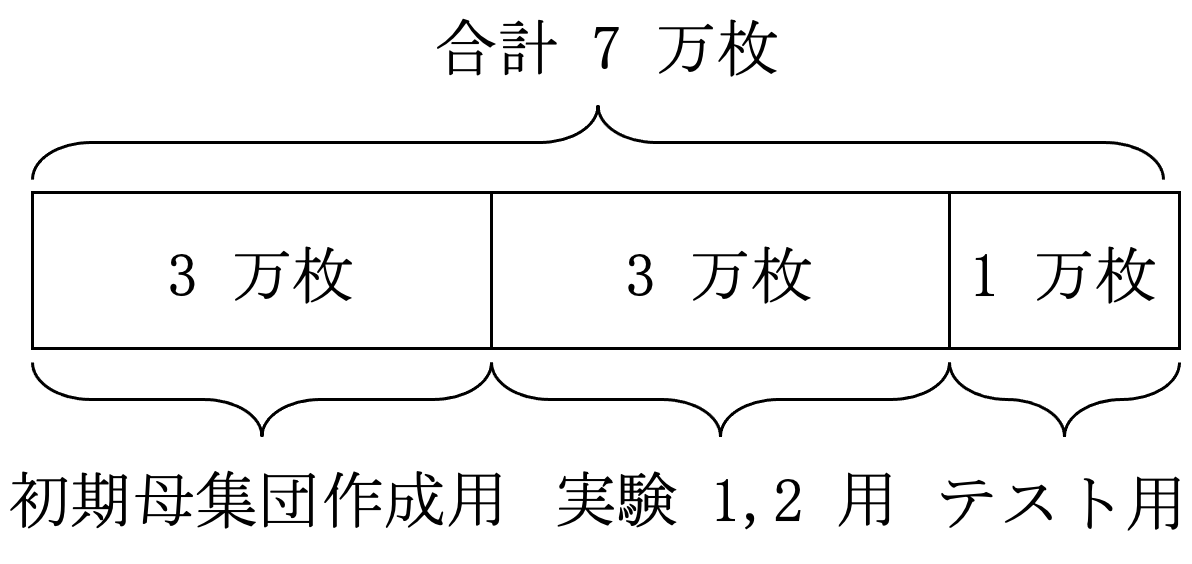
\includegraphics[height=4cm]{dataset_devide.png}
    \caption{データセットの分割}
    \label{dataset}
\end{figure}

\begin{table}[ht]
    \centering
    \caption{実験 1,2 実験条件}
    \begin{tabular}{|c|c|}
        \hline
        個体数&100 \\ \hline
        層数&10 \\ \hline
        最小全結合層数&1 \\ \hline
        最大全結合数&3 \\ \hline
        選択割合&40 \\ \hline
        交叉割合&40 \\ \hline
        突然変異割合&20 \\ \hline
        本学習エポック数&100 \\ \hline
        探索バッチサイズ&24 \\ \hline
        本学習バッチサイズ&16 \\ \hline
        学習率&1e-4 \\ \hline
        最適化手法&Adam \\ \hline
        温度&0.04 \\ \hline
    \end{tabular}
    \label{tab1}
\end{table}

\section{実験結果}

\subsection{実験用初期個体群の作成}
探索前の個体群の適応度の平均値は 63.26 \% で,20 世代探索後の個体群の適応度の平均値は 85.64 \% となっており,上昇していることが確認できる.そのため当初の,後の実験の時間短縮という目的の達成が見込まれる.よって以下の実験 1 ,2 では,ここで作成した個体群を初期個体群として採用した.
%適応度の推移のグラフと,最終的な適応度のmeanを提示.

\subsection{実験 1 の結果}
表 \ref{実験1_結果} に作成した初期母集団を用いて,$c = 80$ として実験をした結果を示す.表 \ref{実験1_結果} の値は,各試行の最終世代において最も適応度が高かったものを 100 エポック本学習させたときの最良識別精度である.表 \ref{実験1_結果} より,エポック数 $n$ と 世代数 $g$ の組 $(n, g)$ が,$(80, 1)$,$(40, 2)$,$(20, 4)$,と,$n$ が増えるにつれて識別精度が良くなり,$(n, g) = (16, 5)$ の時にピークを迎え,その後は識別精度は悪化していったことが読み取れる.これはエポック数を適切に増やして学習すると,将来的な性能が予測しやすくなるためと考える.

% \begin{table}[ht]
%     \centering
%     \caption{実験 1 の結果}
%     \begin{tabular}{|c|c|c|c|c|}
%         \hline
%         $g$&$n$& 1 回目 [\%]& 2 回目 [\%]&平均値 [\%] \\ \hline
%         80&1&92.04&89.42&90.73 \\ \hline
%         40&2&92.13&& \\ \hline
%         20&4&92.26&& \\ \hline
%         16&5&93.09&& \\ \hline
%         10&8&90.00&& \\ \hline
%         8&10&92.29&& \\ \hline
%     \end{tabular}
%     \label{実験1_結果}
% \end{table}

\begin{table}[ht]
    \centering
    \caption{実験 1 の結果}
    \begin{tabular}{|c|c|c|c|c|}
        \hline
        世代数&エポック数&識別精度 [\%] \\ \hline
        80&1&92.04 \\ \hline
        40&2&92.13 \\ \hline
        20&4&92.26 \\ \hline
        16&5&93.09 \\ \hline
        10&8&90.00 \\ \hline
        8&10&92.29 \\ \hline
    \end{tabular}
    \label{実験1_結果}
\end{table}

\subsection{実験 2 の結果}
表 \ref{実験2_結果} に実験 2 の結果を示す.表 \ref{実験2_結果} から,探索フェーズ終盤にエポック数を大きくした方がより良い個体を得ることができるということが確認できる.探索終盤に本学習に相対的に近いエポック数で学習することで,本学習したときにより良い精度となる個体を選択できたと考えられる.

\begin{table}[ht]
    \centering
    \caption{実験 2 の結果}
    \begin{tabular}{|c|c|c|c|}
        \hline
        条件& 1 回目 [\%]& 2 回目 [\%]&平均値 [\%] \\ \hline
        $n$ 増加&91.91&92.39&92.15 \\ \hline
        $n$ 減少&91.34&91.96&91.65 \\ \hline
    \end{tabular}
    \label{実験2_結果}
\end{table}

\section{まとめと今後の課題}
本実験では,tdgaCNN における適応度評価を様々な方法で実験し,それが得られる CNN の精度にどのような影響を及ぼすかを調査した.その結果として,1 エポックのみ学習させた時の精度を適応度としたときよりも,適切なエポック数を定め,そのエポック数で学習させた時の精度を適応度とした時の方が良い個体が得られるという結果が得られた.また,探索序盤よりも探索終盤に適応度評価のための学習エポック数を増やす方が,より良い個体が得られるということも確かめられた.\par
今後の課題として,試行回数を増やすことで,適応度評価手法ごとの信頼区間を調査することが挙げられる.また本実験で,適応度評価のための学習エポック数を変化させると,得られる個体の良し悪しに影響を及ぼすということは確認できたが,そのエポック数をどのように最適化するかということについては解明できていない.様々な実験条件下で,エポック数を最適化する手法を提案することも,今後の課題である.
%また,適切な温度スケジューリングを施すことも今後の課題の一つである.今回は,tdgaCNN における温度を 0.04 と一定値として実験をした.温度は,世代の多様性をどの程度維持するかを決める大切なパラメータであり,探索序盤,中盤,そして後半にかけて,変化させていくことによって,より適切に多様性を維持した探索をすることができると考える.

\bibliography{index}
\bibliographystyle{junsrt} %参考文献出力スタイル
\end{document}
